\documentclass[10pt,journal,compsoc]{IEEEtran}

% ===================== Packages =====================
\usepackage{graphicx}
\usepackage{tabularx}
\usepackage{amsmath}
\usepackage{amsthm}
\usepackage{amssymb}
\usepackage{booktabs}
\usepackage{cite}
\usepackage{url}
\usepackage[hidelinks]{hyperref}
\usepackage{xcolor}
\usepackage{array}

% ===================== Theorem Environments =====================
\newtheorem{theorem}{Theorem}[section]
\newtheorem{lemma}[theorem]{Lemma}
\newtheorem{corollary}[theorem]{Corollary}
\newtheorem{proposition}[theorem]{Proposition}
\newtheorem{definition}[theorem]{Definition}
\newtheorem{assumption}[theorem]{Assumption}
\theoremstyle{remark}
\newtheorem{remark}{Remark}[section]

% ===================== Bibliography =====================

% ===================== Metadata =====================
\title{Scarcity Is Not Enough: An Impossibility Result for\\
	Linear Sybil Cost Under Parallelizable Resources}

\author{Homayoun Maleki,~\IEEEmembership{}
	Nekane Sainz,~\IEEEmembership{}
	Jon Legarda,~\IEEEmembership{}
	and~Igor Santos-Grueiro~\IEEEmembership{}
	\IEEEcompsocitemizethanks{
		\IEEEcompsocthanksitem H. Maleki, N. Sainz, and J. Legarda are with
		DeustoTech, University of Deusto, Bilbao, Spain.
		E-mail: h.maleki@deusto.es
		\IEEEcompsocthanksitem I. Santos-Grueiro is with the International
		University of La Rioja (UNIR), Logroño, Spain.
}}

\begin{document}
	
	\maketitle
	
	% -------------------------------------------------------
	%  ABSTRACT
	% -------------------------------------------------------
	\begin{abstract}
		Permissionless systems resist Sybil attacks by binding influence
		to scarce resources.
		We show that scarcity alone is insufficient: the structural
		properties of the resource determine whether influence can be
		concentrated at sublinear cost---whether through identity
		replication, delegation, or pooling.
		
		We model this through the adversarial cost $C(s,T)$: the minimum
		expenditure required to achieve influence proportional to $s$
		independent participation units over $T$ windows.
		We prove that any resource satisfying divisibility, additivity
		of influence, temporal reusability, and identity transferability
		admits \emph{influence amortization}: $C(s,T) = o(sT)$,
		regardless of protocol design.
		This is an impossibility result---no protocol rule can enforce
		linear cost of influence concentration over a structurally
		parallelizable resource.
		
		We further prove that throughput-bounded, non-transferable,
		window-local resources enforce $C(s,T) = \Omega(sT)$: each
		additional unit of sustained influence incurs marginal cost
		$\Delta(s,T) = \Omega(T)$, growing with the time horizon.
		The two resource classes are asymptotically separated.
		
		As a direct design consequence, any mechanism targeting linear
		cost of influence concentration must ground participation in a
		resource that violates at least one parallelizability property.
	\end{abstract}
	
	\begin{IEEEkeywords}
		Sybil resistance, influence concentration, parallelizable resources,
		throughput-bounded resources, adversarial cost scaling,
		structural impossibility, permissionless systems
	\end{IEEEkeywords}
	
	% -------------------------------------------------------
	%  I. INTRODUCTION
	% -------------------------------------------------------
	\section{Introduction}
	\label{sec:intro}
	
	Permissionless systems rest on a radical premise: that open
	participation, without gatekeepers or trusted authorities,
	can produce secure and fair collective outcomes.
	The mechanism that makes this possible---binding influence
	to the expenditure of a scarce resource---has been the
	cornerstone of distributed consensus since
	Nakamoto~\cite{nakamoto2008bitcoin}.
	Yet deployment has revealed a persistent gap between
	this promise and reality.
	Bitcoin's hash power is concentrated in a handful of
	mining pools~\cite{gencer2018decentralization}.
	Ethereum's stake is dominated by a small number of
	liquid staking providers~\cite{lido2023concentration}.
	
	This paper identifies the structural reason why.
	
	\subsection{Resource-Based Defenses and Their Shared Blind Spot}
	\label{ssec:sybil}
	
	The foundational obstacle in permissionless systems is the
	Sybil attack~\cite{douceur2002sybil}: a single adversary
	generates many identities to amplify influence beyond any
	honest participant.
	The standard response is to make identity costly by tying
	participation to a scarce resource.
	Proof-of-Work binds influence to computational
	effort~\cite{nakamoto2008bitcoin,garay2015backbone}.
	Proof-of-Stake binds it to financial
	capital~\cite{kiayias2017ouroboros}.
	Graph-based defenses~\cite{yu2006sybilguard,yu2008sybillimit}
	constrain identity placement via social structure.
	Identity-binding mechanisms~\cite{borge2017pop,ford2020pseudonym}
	restrict credential issuance to verified participants.
	
	Despite their diversity, these approaches share a common
	blind spot.
	The original insight behind resource-weighted
	participation---introduced by Proof-of-Work---was
	precise: binding influence to a scarce resource
	prevents cheap identity creation from amplifying
	adversarial power.
	Subsequent work has studied this principle extensively,
	asking whether an adversary's \emph{aggregate} resource
	share crosses a safety threshold.
	
	What has received far less attention is a different
	question: does the \emph{structure} of that resource
	permit influence to be concentrated at sublinear cost?
	A resource that is divisible, transferable, and reusable
	allows a fixed base to be redistributed---through
	identity replication, delegation, or pooling---achieving
	disproportionate influence without proportional expenditure,
	even when aggregate resource share remains unchanged.
	This paper characterizes exactly which resource properties
	permit this concentration, and which ones prevent it.
	
	\subsection{Why Concentration Is Structurally Inevitable}
	\label{ssec:concentration}
	
	The concentration patterns observed across deployed systems
	are not protocol failures.
	They are structural consequences of the resources those
	protocols are built on.
	
	In Bitcoin, mining pools aggregate hash power from thousands
	of participants into a small number of coordinated identities.
	Gencer et al.~\cite{gencer2018decentralization} document
	that the top-four pools routinely control over fifty percent
	of total hash power.
	The reason is structural: computational capacity is
	\emph{divisible}, \emph{transferable}, and \emph{temporally
		reusable}---properties that allow a fixed resource base to
	be aggregated, redistributed, and reused across arbitrarily
	many identities at vanishing marginal
	cost~\cite{rosenfeld2011analysis,bonneau2015sok}.
	Moreover, influence is \emph{additive}: distributing $r$
	across $k$ identities preserves total influence,
	$\sum_{i} f(r_i) = f(r)$, so redistribution incurs no
	penalty.
	
	Proof-of-Stake replaced computational effort with
	financial capital, eliminating PoW's energy cost.
	But the structure of the underlying resource is
	identical in the relevant sense: capital is divisible,
	transferable, temporally reusable, and additive in influence.
	Delegation mechanisms allow a fixed capital base to be
	distributed across many validator identities, each carrying
	proportional influence~\cite{kiayias2017ouroboros,saleh2021blockchain}.
	The outcome is familiar: as of 2023, Lido Finance alone
	controlled approximately thirty percent of all staked
	ETH~\cite{lido2023concentration}.
	
	The same structural argument applies to every resource
	that can be subdivided and reused across identities.
	The pattern is not a coincidence.
	When a resource satisfies all four properties, a fixed
	base can be aggregated and redistributed across arbitrarily
	many identities---amplifying network presence, proposal
	bandwidth, and committee weight without proportional
	expenditure.
	The concentration of power is not an externality.
	It is built into the resource.
	
	\subsection{The Missing Question}
	\label{ssec:missing}
	
	The observation above points to a question existing
	analyses do not answer:
	
	\begin{quote}
		\emph{What structural properties of a security resource
			guarantee that no adversary can achieve $s$-unit influence
			over $T$ windows at cost below $\Omega(sT)$?}
	\end{quote}
	
	We formalize this through $C(s,T)$: the minimum
	expenditure required to achieve influence proportional
	to $s$ independent participation units over $T$
	consecutive windows---whether through identity
	replication, delegation, or pooling.
	Two regimes matter.
	If $C(s,T) = o(sT)$, a fixed resource base suffices
	to achieve arbitrarily large influence---concentration
	is cheap regardless of protocol design.
	If $C(s,T) = \Omega(sT)$, each additional unit of
	sustained influence requires proportional expenditure---
	concentration is structurally infeasible.
	
	The answer, we show, is determined entirely by the
	\emph{structure} of the underlying resource.
	No protocol rule can enforce $C(s,T) = \Omega(sT)$
	when the resource itself is divisible, transferable,
	temporally reusable, and additive in influence.
	This is an impossibility result.
	It holds independently of consensus design, cryptographic
	assumptions, or network model.
	
	But impossibility alone is not enough.
	The second result of this paper is constructive:
	we identify a class of resources---throughput-bounded,
	non-transferable, and window-local---that
	\emph{provably enforces} $C(s,T) = \Omega(sT)$.
	This resource class has not been formally characterized
	in prior work.
	Beyond its theoretical significance, this characterization
	is actionable: Any consensus protocol grounded in a throughput-bounded,
	non-transferable, and window-local resource inherits
	$C(s,T) = \Omega(sT)$ by construction, without additional protocol-level
	enforcement.
	Introducing this class, and proving its properties,
	is the central contribution of this paper.
	
	\subsection{This Paper}
	\label{ssec:thispaper}
	
	This paper draws a structural boundary in the design space
	of permissionless systems and introduces a resource class
	that sits on the right side of it.
	
	We prove that any resource satisfying four properties---
	divisibility, additivity of influence, temporal reusability,
	and identity transferability---admits \emph{influence
		amortization}: $C(s,T) = o(sT)$, regardless of protocol
	design.
	Computation, capital, storage, and delegated stake all
	fall into this class.
	No mechanism built on such a resource can enforce linear
	cost of influence concentration.
	
	We then introduce \emph{throughput-bounded resources}:
	resources in which each participation unit requires an
	independent channel, the channel output is non-transferable,
	and allocation does not carry over across time windows.
	We prove that any such resource enforces
	$C(s,T) = \Omega(sT)$: each additional unit of sustained
	influence incurs marginal cost $\Delta(s,T) = \Omega(T)$,
	growing with the time horizon.
	Concentration of influence is structurally infeasible
	by construction.
	
	Together, these two results establish a sharp asymptotic
	separation: parallelizable resources admit influence
	concentration at vanishing marginal cost; throughput-bounded
	resources structurally preclude it.
	
	The separation between these two classes yields a direct
	design rule---the \emph{Resource Substitution Principle}:
	enforcing linear cost of influence concentration requires
	grounding participation in a resource that violates at
	least one parallelizability property.
	Protocol design cannot substitute for resource structure.
	
	\subsection{Contributions}
	\label{ssec:contributions}
	
	\begin{enumerate}
		
		\item \textbf{Impossibility under parallelizable resources
			(Theorem~\ref{thm:impossible}).}
		Any mechanism whose weighting resource satisfies
		divisibility, additivity, temporal reusability, and
		identity transferability satisfies $C(s,T) = o(sT)$,
		regardless of protocol design.
		Influence concentration is achievable at vanishing
		marginal cost.
		
		\item \textbf{Linear cost of influence concentration under
			throughput-bounded resources (Theorem~\ref{thm:linear}).}
		We introduce the class of throughput-bounded,
		non-transferable, window-local resources and prove
		that any such resource enforces $C(s,T) = \Omega(sT)$,
		with marginal cost $\Delta(s,T) = \Omega(T)$.
		
		\item \textbf{Resource Substitution Principle
			(Theorem~\ref{thm:substitution}).}
		Linear cost of influence concentration requires
		violating at least one parallelizability property.
		No protocol can enforce this boundary without a
		structural change in the underlying resource.
		
	\end{enumerate}
	
	\subsection{Paper Organization}
	\label{ssec:organization}
	
	Section~\ref{sec:related} reviews related work.
	Section~\ref{sec:model} presents the system model.
	Section~\ref{sec:framework} develops the resource framework.
	Section~\ref{sec:impossibility} proves the impossibility result.
	Section~\ref{sec:lowerbound} proves the linear lower bound.
	Section~\ref{sec:separation} establishes the structural
	separation, the Resource Substitution Principle,
	and hybrid system behavior.
	Section~\ref{sec:instantiations} classifies concrete resource types.
	Section~\ref{sec:evaluation} presents the evaluation.
	Section~\ref{sec:limitations} discusses limitations.
	Section~\ref{sec:conclusion} concludes.
	
	% -------------------------------------------------------
	%  II. RELATED WORK
	% -------------------------------------------------------
	\section{Related Work}
	\label{sec:related}
	
	Prior work on Sybil resistance and permissionless systems
	addresses several distinct security questions.
	We survey the main research directions and identify
	the gap this paper fills.
	Table~\ref{tab:positioning} summarizes the distinction.
	
	\subsection{Resource-Based Sybil Defenses}
	\label{ssec:rw_resource}
	
	Douceur~\cite{douceur2002sybil} established that in the
	absence of a trusted authority, identity replication in
	open systems cannot be prevented.
	Nakamoto~\cite{nakamoto2008bitcoin} proposed binding
	participation to a scarce resource---computational
	effort---as a practical response to this impossibility.
	Formal analyses of Nakamoto-style
	consensus~\cite{garay2015backbone,ren2019nakamoto,pass2017hybrid,pass2017fruitchains}
	establish chain-growth, common-prefix, and chain-quality
	guarantees expressed as thresholds on adversarial hash power.
	Proof-of-Stake protocols---including
	Ouroboros~\cite{kiayias2017ouroboros,kiayias2018ouroboros,kiayias2020genesis},
	Snow White~\cite{pass2016snowwhite},
	and Algorand~\cite{gilad2017algorand}---replace
	computational effort with financial capital and derive
	analogous guarantees as thresholds on adversarial stake.
	These protocols collectively instantiate the
	aggregate-threshold adversarial model formalized in
	foundational Byzantine fault-tolerance
	work~\cite{lamport1982byzantine,castro1999pbft};
	Algorand additionally employs verifiable random
	functions~\cite{micali1999vrf} for committee selection.
	
	These analyses consistently reason about
	\emph{aggregate} adversarial resource ownership.
	Security guarantees take the form: if the adversary
	controls less than a threshold fraction of the total
	resource, the protocol is safe.
	They do not characterize whether a fixed resource base
	can be used to concentrate influence at sublinear
	marginal cost.
	The present paper addresses this question directly.
	
	\subsection{Empirical and Systems-Level Analyses}
	\label{ssec:rw_empirical}
	
	Empirical work documents the centralization patterns
	that resource-based mechanisms produce in practice.
	Gencer et al.~\cite{gencer2018decentralization} measure
	mining pool concentration in Bitcoin and Ethereum.
	Rosenfeld~\cite{rosenfeld2011analysis,rosenfeld2014analysis}
	analyzes pooled mining reward systems and hash-rate-based
	double-spending dynamics.
	Bonneau et al.~\cite{bonneau2015sok} and
	Narayanan et al.~\cite{narayanan2016bitcoinbook} survey
	the broader security and deployment landscape of Bitcoin.
	Gervais et al.~\cite{gervais2016security,gervais2014isbitcoin}
	quantify security-performance tradeoffs and decentralization
	properties of deployed proof-of-work systems.
	Work on selfish mining~\cite{eyal2014majority} and
	double-spending~\cite{kroll2013economics} analyzes
	adversarial strategies under aggregate resource models.
	Network-layer studies~\cite{neudecker2019network} document
	how propagation dynamics interact with pool-driven
	resource concentration.
	
	These works describe the \emph{symptoms} of structural
	resource properties---concentration, pooling, delegation---
	but do not formally characterize why such patterns are
	structurally inevitable under divisible, reusable resources.
	The present paper provides this characterization.
	
	\subsection{Economic Analyses of Consensus}
	\label{ssec:rw_economic}
	
	Budish~\cite{budish2018economic} and
	Budish et al.~\cite{budish2024economic} analyze the
	economic limits of permissionless consensus, framing
	security in terms of the cost of mounting a majority attack.
	Carlsten et al.~\cite{carlsten2016instability} study
	incentive stability in the absence of block rewards.
	Saleh~\cite{saleh2021blockchain} provides an equilibrium
	analysis of Proof-of-Stake.
	
	These analyses model adversarial capability in terms of
	aggregate resource ownership and study equilibrium
	incentives or corruption costs.
	They do not study whether influence can be concentrated
	at sublinear cost through delegation or pooling---the
	question central to this paper.
	
	\subsection{Graph-Based and Social-Structure Defenses}
	\label{ssec:rw_graph}
	
	SybilGuard~\cite{yu2006sybilguard},
	SybilLimit~\cite{yu2008sybillimit}, and
	SybilControl~\cite{li2017sybilcontrol} bound adversarial
	influence by exploiting the observation that in social
	networks, the number of edges between honest and Sybil
	regions is small relative to internal connectivity.
	SybilInfer~\cite{danezis2009sybilinfer} applies
	probabilistic inference over trust graphs to identify
	adversarial clusters.
	Game-theoretic analyses~\cite{lesniewski2020analysis}
	study equilibrium conditions under which honest participants
	can deter adversarial identity creation.
	
	These approaches address a different question: where
	Sybil identities can be placed within a social graph,
	rather than how the cost of adversarial influence scales
	over time.
	They provide no characterization of $C(s,T)$ as $s$
	or $T$ grows, and their guarantees depend on
	graph-topology assumptions that may not hold in
	practice~\cite{wang2019attack}.
	
	\subsection{Identity-Binding Mechanisms}
	\label{ssec:rw_identity}
	
	Proof-of-Personhood~\cite{borge2017pop} and pseudonym
	parties~\cite{ford2020pseudonym} bind credentials to
	real-world participants to enforce one-person--one-identity
	mappings.
	Reputation systems~\cite{resnick2000reputation} offer a
	related but distinct approach: rather than binding
	participation to verified identity, they tie influence
	to accumulated behavioral history.
	These mechanisms address \emph{admission}---restricting
	the creation of new identities---rather than the sustained
	cost of concentrating influence over time.
	Once admitted, influence may still be governed by a
	transferable, reusable resource.
	
	\subsection{Capability and Rate-Limiting Architectures}
	\label{ssec:rw_capability}
	
	Hardware-rooted execution environments such as
	Intel SGX~\cite{costan2016intel} enforce per-device
	participation limits that bind resource generation
	to specific hardware.
	Capability-based systems~\cite{levy1984capability}
	and congestion-control mechanisms~\cite{jacobson1988congestion}
	impose per-actor throughput constraints in different
	deployment contexts.
	Bitcoin-NG~\cite{eyal2018bitcoinng} decouples block
	leadership from transaction throughput, instantiating
	a per-leader rate constraint as a protocol-level primitive.
	HoneyBadger BFT~\cite{miller2016honeybadger} makes
	explicit throughput bounds central to its communication
	complexity analysis.
	Alwen et al.~\cite{alwen2019blockchain} study
	sustained space and time complexity of sequential
	proof-of-work constructions.
	
	These works impose per-actor throughput constraints
	but analyze them in the context of access control,
	network stability, or computational hardness---not
	the cost of influence concentration.
	They do not establish the structural separation between
	parallelizable and throughput-bounded resource classes
	that this paper proves.
	
	\subsection{Positioning}
	\label{ssec:rw_positioning}
	
	The common thread across prior work is a focus on
	\emph{aggregate} adversarial capability: how much
	resource does an adversary control, and is it below
	a safety threshold?
	No prior work asks whether a fixed aggregate resource
	can be used to concentrate influence at sublinear
	marginal cost---whether through identity replication,
	delegation, or pooling---nor establishes the structural
	conditions under which this is or is not possible.
	
	This paper provides that characterization.
	We identify the structural properties that determine
	whether adversarial cost scales as $o(sT)$ or
	$\Omega(sT)$, establish an impossibility result for
	parallelizable resources, introduce the throughput-bounded
	resource class and prove its linear cost guarantee,
	and derive a design principle for systems requiring
	linear cost of influence concentration.
	
	\begin{table*}[t]
		\caption{Positioning of This Work Relative to Prior Literature}
		\label{tab:positioning}
		\centering
		\renewcommand{\arraystretch}{1.4}
		\begin{tabularx}{\textwidth}{@{}p{3.8cm}Xp{4.5cm}c@{}}
			\toprule
			\textbf{Research Line} & \textbf{Representative Works} & \textbf{Primary Security Question} & \textbf{Influence} \\
			&                               &                                    & \textbf{Concentration Cost?} \\
			\midrule
			Sybil attack literature
			& \cite{douceur2002sybil,yu2006sybilguard,yu2008sybillimit,danezis2009sybilinfer}
			& Can adversaries create multiple identities, and how can identity creation be restricted or detected?
			& No \\[4pt]
			Blockchain consensus security
			& \cite{lamport1982byzantine,castro1999pbft,garay2015backbone,ren2019nakamoto,kiayias2017ouroboros,gilad2017algorand}
			& Under what aggregate adversarial resource ownership do safety and liveness properties fail?
			& No \\[4pt]
			Economic analyses of consensus
			& \cite{budish2018economic,budish2024economic,kroll2013economics}
			& What equilibrium incentives and corruption costs arise in resource-weighted consensus?
			& No \\[4pt]
			Graph-based defenses
			& \cite{yu2006sybilguard,yu2008sybillimit,danezis2009sybilinfer}
			& Can Sybil proliferation be constrained via social-network structure?
			& No \\[4pt]
			Identity-binding mechanisms
			& \cite{borge2017pop,ford2020pseudonym}
			& How can systems enforce one-person--one-identity mappings?
			& No \\[4pt]
			Capability / rate-limiting architectures
			& \cite{costan2016intel,levy1984capability,jacobson1988congestion}
			& Can per-actor throughput limits be enforced at the system level?
			& No \\
			\midrule
			\textbf{This paper}
			& ---
			& How do structural properties of security resources determine whether influence can be concentrated at sublinear cost?
			& \textbf{Yes} \\
			\bottomrule
		\end{tabularx}
	\end{table*}
	
	% -------------------------------------------------------
	%  III. SYSTEM MODEL
	% -------------------------------------------------------
	\section{System Model}
	\label{sec:model}
	
	We model an open and permissionless system in which
	identity creation is inexpensive and no admission
	authority exists.
	Influence is regulated by a security-weighting resource
	$\mathcal{R}$.
	Our objective is to characterize how structural properties
	of $\mathcal{R}$ determine whether influence can be
	concentrated at sublinear cost---whether through identity
	replication, delegation, or pooling.
	
	Table~\ref{tab:notation} summarizes the core notation.
	
	\subsection{Identities and Participation}
	\label{ssec:identity}
	
	In permissionless systems, an identity is a cryptographic
	key pair that authorizes participation.
	A single real-world entity may control arbitrarily many
	key pairs, and therefore arbitrarily many identities,
	at negligible cost~\cite{douceur2002sybil}.
	Influence concentration may therefore arise either through
	\emph{identity replication}---controlling many key pairs
	each with unit weight---or through \emph{resource
		aggregation}---controlling few key pairs but delegating
	or pooling sufficient resource to achieve equivalent
	aggregate influence.
	The model captures both mechanisms uniformly.
	
	Let $\mathcal{U}$ denote the universe of potential
	participants.
	At each time window $t$, the system contains a set of
	active identities $\mathcal{V}_t \subseteq \mathcal{U}$.
	An adversary $\mathcal{A}$ is \emph{identity-unbounded}:
	it may create, retire, and coordinate an arbitrary
	number of identities at negligible syntactic cost.
	Let $S_t \subseteq \mathcal{V}_t$ denote the set of
	identities controlled by $\mathcal{A}$ at window $t$,
	with $|S_t| = s_t$.
	No a priori bound is placed on $s_t$.
	
	\subsection{Time Model}
	\label{ssec:time}
	
	Time proceeds in discrete windows $t = 1, 2, \ldots$
	A window represents the minimal interval over which
	resource allocation and influence are refreshed---for
	example, a block interval or governance epoch.
	
	We evaluate security over a finite horizon of $T$
	windows.
	An identity is \emph{sustained} if it remains active
	throughout all windows $t = 1, \ldots, T$.
	
	\subsection{Resource and Influence}
	\label{ssec:resource}
	
	Let $\mathcal{R}$ denote the security-weighting resource.
	For each identity $v \in \mathcal{V}_t$ and window $t$,
	let $r_v(t) \in \mathbb{R}_{\geq 0}$ denote the
	resource allocated to $v$.
	Influence is determined by a mapping
	\begin{equation}
		W_v(t) = f\bigl(r_v(t)\bigr),
	\end{equation}
	where $f : \mathbb{R}_{\geq 0} \to \mathbb{R}_{\geq 0}$
	is the protocol's resource-to-influence function.
	No structural assumptions are placed on $f$ at this
	stage; these will be derived from properties of
	$\mathcal{R}$ in Section~\ref{sec:framework}.
	
	The total adversarial influence at window $t$ is
	\begin{equation}
		W_{\mathcal{A}}(t) = \sum_{v \in S_t} W_v(t).
	\end{equation}
	
	\begin{definition}[Activation Threshold]
		\label{def:threshold}
		There exists a constant $r_{\min} > 0$ such that
		an identity is active in window $t$ only if
		$r_v(t) \geq r_{\min}$.
	\end{definition}
	
	\begin{remark}[Structural interpretation of $r_{\min}$]
		\label{rem:rmin}
		$r_{\min}$ is a structural property of the resource
		deployment, not a free protocol parameter.
		In Proof-of-Work, it corresponds to the minimum
		computational contribution required to produce a valid
		share within a window---a constraint of the hardware
		and difficulty setting.
		In device-bound execution, it is the minimum attestation
		output a device must generate to register as active.
		A protocol setting $r_{\min} = 0$ admits zero-resource
		identities, which produce zero influence ($f(0) = 0$)
		and contribute nothing to $W_{\mathcal{A}}(t)$; this
		is a degenerate case outside the model scope.
		For deployments where $r_{\min}$ is design-dependent,
		Theorem~\ref{thm:linear} gives a lower bound
		parameterized by the deployment's participation floor:
		$C(s,T) \geq s \cdot T \cdot r_{\min}$ holds for any
		fixed $r_{\min} > 0$ and is non-vacuous whenever a
		positive participation threshold is enforced.
	\end{remark}
	
	The activation threshold establishes a per-identity,
	per-window resource floor that is unavoidable regardless
	of resource structure.
	The structural results of this paper concern costs
	\emph{beyond} this floor: whether a resource imposes
	an additional $T$-scaling cost per unit of sustained
	influence, or whether temporal reusability eliminates it.
	
	\subsection{Adversarial Model}
	\label{ssec:adversary}
	
	The adversary $\mathcal{A}$ is computationally
	unbounded but constrained by the structural
	properties of $\mathcal{R}$.
	Specifically, $\mathcal{A}$ may:
	\begin{itemize}
		\item instantiate, retire, and coordinate
		an arbitrary number of identities;
		\item allocate and reallocate resource across
		identities when the resource structure permits;
		\item reuse resource across time windows when
		temporal reuse is allowed;
		\item aggregate influence through delegation
		or pooling when the resource structure permits.
	\end{itemize}
	
	This model subsumes the aggregate-resource adversaries
	used in blockchain consensus
	analyses~\cite{garay2015backbone,kiayias2017ouroboros}
	while remaining protocol-agnostic.
	The adversary's only binding constraint is the
	structural properties of $\mathcal{R}$, formalized
	in Section~\ref{sec:framework}.
	
	\subsection{Adversarial Cost}
	\label{ssec:cost}
	
	\begin{definition}[Adversarial Cost Function]
		\label{def:cost}
		Let $R_{\mathcal{A}}(t) = \sum_{v \in S_t} r_v(t)$
		denote the total resource expenditure of $\mathcal{A}$
		at window $t$, and let $W_{\mathrm{unit}} = f(r_{\min})$
		denote the influence of an identity operating at the
		activation threshold.
		$C(s, T)$ denotes the minimum total resource
		expenditure required to achieve influence proportional
		to $s$ independent participation units over $T$
		consecutive windows---whether through sustaining
		$s$ active identities, delegating to $s$ validators,
		pooling toward equivalent aggregate weight, or any
		combination thereof:
		\begin{equation}
			C(s, T) \;=\; \inf \left\{
			\sum_{t=1}^{T} R_{\mathcal{A}}(t)
			\;\Bigg|\;
			\begin{array}{l}
				W_{\mathcal{A}}(t) \geq s \cdot W_{\mathrm{unit}} \\[3pt]
				\forall\, t \in \{1,\ldots,T\}
			\end{array}
			\right\}.
		\end{equation}
	\end{definition}
	
	This definition captures influence concentration in
	full generality: the adversary may achieve influence
	proportional to $s$ units through any combination
	of identity replication, resource delegation, or
	pooling, whichever minimizes total expenditure.
	
	To expose the structure of costs, we decompose
	$C(s, T)$ as
	\begin{equation}
		C(s, T) = C_{\mathrm{stock}}(s)
		+ C_{\mathrm{flow}}(s, T)
		+ h(s, T),
	\end{equation}
	where $C_{\mathrm{stock}}(s)$ is the one-time
	acquisition cost of resources that persist across
	all $T$ windows without renewal (e.g., staked capital,
	hardware); $C_{\mathrm{flow}}(s, T)$ is the cumulative
	per-window expenditure for resources that must be
	renewed each window (e.g., energy, device attestations);
	and $h(s, T)$ is the coordination overhead of managing
	$s$ participation units over $T$ windows.
	
	The structural separation of
	Sections~\ref{sec:impossibility}--\ref{sec:lowerbound}
	concerns the scaling of $C_{\mathrm{flow}}(s, T)$:
	parallelizable resources admit
	$C_{\mathrm{flow}}(s, T) = 0$ once stock is acquired,
	whereas throughput-bounded resources enforce
	$C_{\mathrm{flow}}(s, T) = \Omega(sT)$.
	
	\begin{assumption}[Amortized Coordination]
		\label{asm:coordination}
		The coordination overhead satisfies $h(s, T) = o(sT)$.
	\end{assumption}
	
	This assumption captures the empirically observed
	behavior of pooling and delegation infrastructure:
	mining pools, validator delegation services, and
	cloud-managed multi-account orchestration each allow
	an operator to manage many participation units with
	overhead scaling as $O(s + T)$ rather than
	$O(sT)$~\cite{rosenfeld2011analysis,bonneau2015sok,
		saleh2021blockchain}.
	Assumption~\ref{asm:coordination} is an environmental
	condition on coordination infrastructure, not a
	property of $\mathcal{R}$; the two are independent.
	Theorem~\ref{thm:impossible} holds even when
	$h(s, T) = 0$, and Theorem~\ref{thm:linear} holds
	regardless of how small $h(s, T)$ is.
	
	\begin{remark}[Boundary case: $h(s,T) = \Omega(sT)$]
		\label{rem:coord_linear}
		Assumption~\ref{asm:coordination} characterizes
		the adversarially favorable regime in which
		coordination is cheap.
		If $h(s,T) = \Omega(sT)$---for example, because
		managing $s$ independent identities requires
		$\Omega(sT)$ communication or operational
		effort---then $C(s,T) \geq h(s,T) = \Omega(sT)$
		holds immediately, independently of resource
		structure.
		In this case the adversary already faces linear
		cost from coordination alone.
		Theorem~\ref{thm:impossible} therefore establishes
		the \emph{worst case for the defender}: even when
		coordination overhead is asymptotically free,
		a parallelizable resource admits $C(s,T) = o(sT)$.
		When coordination is not free, the adversary's
		position is no better.
	\end{remark}
	
	\subsection{Scaling Regimes}
	\label{ssec:regimes}
	
	Two asymptotic regimes characterize the adversarial
	cost function.
	
	\begin{definition}[Scaling Regimes]
		\label{def:regimes}
		A mechanism exhibits \emph{sublinear scaling} if
		$C(s, T) = o(sT)$, and \emph{linear scaling} if
		$C(s, T) = \Omega(sT)$.
	\end{definition}
	
	Under sublinear scaling, the marginal cost of each
	additional unit of sustained influence does not grow
	with the time horizon:
	$\Delta(s, T) = o(T)$,
	where $\Delta(s, T) = C(s, T) - C(s-1, T)$.
	A fixed resource base suffices to achieve arbitrarily
	large influence---concentration is cheap regardless
	of protocol design.
	
	Under linear scaling, each additional unit of sustained
	influence incurs cost at least $\Omega(T)$, growing
	with the time horizon.
	Achieving influence proportional to $s$ units over
	$T$ windows costs at least $\Omega(sT)$ regardless
	of how the adversary distributes its resource.
	
	The central question of this paper is: which regime
	does a given resource $\mathcal{R}$ induce?
	Section~\ref{sec:framework} provides the structural
	answer.
	
	\begin{table}[t]
		\caption{Core Notation}
		\label{tab:notation}
		\centering
		\renewcommand{\arraystretch}{1.25}
		\begin{tabular}{@{}ll@{}}
			\toprule
			\textbf{Symbol} & \textbf{Meaning} \\
			\midrule
			$v$                  & Identity (key pair / participant instance) \\
			$t$                  & Time window index \\
			$T$                  & Time horizon (number of windows) \\
			$s$                  & Number of independent participation units \\
			$r_v(t)$             & Resource allocated to identity $v$ at window $t$ \\
			$R_{\mathcal{A}}(t)$ & Total adversarial resource at window $t$: $\sum_{v \in S_t} r_v(t)$ \\
			$W_v(t)$             & Influence of identity $v$ at window $t$ \\
			$W_{\mathrm{unit}}$  & Baseline influence: $f(r_{\min})$ \\
			$f(\cdot)$           & Resource-to-influence mapping \\
			$S_t$                & Set of adversarial identities at window $t$ \\
			$C(s,T)$             & Min.\ cost to achieve $s$-unit influence over $T$ windows \\
			$\Delta(s,T)$        & Marginal cost: $C(s,T) - C(s-1,T)$ \\
			$r_{\min}$           & Activation threshold \\
			$\tau$               & Per-channel throughput bound \\
			$h(s,T)$             & Coordination overhead \\
			\bottomrule
		\end{tabular}
	\end{table}
	
	% -------------------------------------------------------
	%  IV. RESOURCE FRAMEWORK
	% -------------------------------------------------------
	\section{Resource Framework}
	\label{sec:framework}
	
	We develop an axiomatic framework for security-weighting
	resources.
	Rather than analyzing specific protocols, we characterize
	resources by their structural properties---the constraints
	they impose on division, aggregation, reuse, and transfer
	across identities and time.
	These properties, not protocol design, determine whether
	influence concentration is achievable at sublinear cost.
	
	%
	% --- A. ---
	%
	\subsection{Resource as a Structural Object}
	\label{ssec:resource_object}
	
	A security-weighting resource $\mathcal{R}$ is a quantity
	that can be allocated across identities, evolves across
	time windows, and determines influence through the
	mapping $f$ of Section~\ref{sec:model}.
	The analysis is agnostic to the semantic nature of
	$\mathcal{R}$---whether it is computation, capital,
	storage, or participation time.
	What matters are the structural properties governing
	how $\mathcal{R}$ behaves under partition, aggregation,
	temporal reuse, and identity transfer.
	
	%
	% --- B. ---
	%
	\subsection{Structural Properties}
	\label{ssec:properties}
	
	\begin{definition}[Divisibility]
		\label{def:divisibility}
		$\mathcal{R}$ is \emph{divisible} if for any allocation
		$r \geq 0$ and integer $k \geq 1$, there exist
		$r_1, \ldots, r_k \geq 0$ with $\sum_{i=1}^{k} r_i = r$,
		and the adversary may distribute $r_i$ to identity $i$
		without additional structural cost.
	\end{definition}
	
	\begin{definition}[Additivity of Influence]
		\label{def:additivity}
		A mechanism \emph{induces additive influence} if
		\begin{equation}
			\sum_{v \in S_t} f\bigl(r_v(t)\bigr)
			\;=\;
			f\!\left(\sum_{v \in S_t} r_v(t)\right).
		\end{equation}
		Total influence depends only on aggregate allocation,
		not on how it is partitioned across identities.
	\end{definition}
	
	\begin{remark}[Scope of Additivity]
		\label{rem:additivity_scope}
		Definition~\ref{def:additivity} is a property of
		the mechanism's influence function $f$, not of
		the resource in isolation.
		It characterizes mechanisms in which influence
		aggregates proportionally with resource allocation.
		This class includes Proof-of-Work (block-production
		probability proportional to hash power),
		linear Proof-of-Stake (voting weight proportional
		to staked capital), and most deployed committee-weight
		and reputation-score protocols.
		Mechanisms deliberately designed to penalize
		concentration---such as quadratic voting, where
		$f(r) = \sqrt{r}$---do not satisfy
		Definition~\ref{def:additivity} and fall outside
		the scope of Theorem~\ref{thm:impossible}.
		The theorem applies precisely to the broad class of
		deployed mechanisms where influence scales with
		aggregate resource share.
	\end{remark}
	
	\begin{definition}[Temporal Reusability]
		\label{def:reusability}
		$\mathcal{R}$ is \emph{temporally reusable} if an
		allocation obtained in window $t$ may be applied in
		window $t+1$ without renewed identity-bound expenditure.
	\end{definition}
	
	\begin{definition}[Identity Transferability]
		\label{def:transferability}
		$\mathcal{R}$ is \emph{identity-transferable} if an
		allocation $r_v(t)$ assigned to identity $v$ may be
		reassigned to any other identity $v'$ without
		proportional cost.
	\end{definition}
	
	\begin{definition}[Throughput-Bounded Resource]
		\label{def:throughput}
		$\mathcal{R}$ is \emph{throughput-bounded} if each
		identity $v$ is associated with a dedicated participation
		channel $C_v$ satisfying all three of the following
		conditions:
		\begin{enumerate}
			\item \emph{Per-channel rate limit.}
			There exists $\tau > 0$ such that
			$r_v(t) \leq \tau$ for all $v$ and $t$.
			\item \emph{Non-transferability.}
			The allocation $r_v(t)$ cannot be simultaneously
			credited to any other identity $v' \neq v$.
			\item \emph{Window-locality.}
			Allocation in window $t$ does not carry over
			to window $t+1$; sustained participation
			requires renewed expenditure in every window.
		\end{enumerate}
	\end{definition}
	
	The three conditions of Definition~\ref{def:throughput}
	jointly imply that each active identity requires an
	independent participation channel whose capacity cannot
	be shared, pooled, or carried forward across identities
	or time.
	Scaling the number of active identities therefore
	requires provisioning additional independent channels.
	
	Note that $\tau$ and $r_{\min}$ are independent
	parameters: $r_{\min}$ is the minimum resource required
	for an identity to be active, while $\tau$ bounds
	the maximum.
	For the system to admit active identities, we require
	$0 < r_{\min} \leq \tau$.
	The linear lower bound of Theorem~\ref{thm:linear}
	holds for any such configuration and is tightest
	when $r_{\min} = \tau$.
	
	%
	% --- C. ---
	%
	\subsection{Resource Classes}
	\label{ssec:classes}
	
	\begin{definition}[Parallelizable Resource]
		\label{def:parallelizable}
		$\mathcal{R}$ is \emph{parallelizable} if it satisfies
		Definitions~\ref{def:divisibility},
		\ref{def:reusability}, and~\ref{def:transferability}
		(divisibility, temporal reusability, and identity
		transferability), and the induced mechanism satisfies
		Definition~\ref{def:additivity} (additivity of
		influence).
	\end{definition}
	
	\begin{definition}[Throughput-Bounded Non-Parallelizable Resource]
		\label{def:nonparallelizable}
		$\mathcal{R}$ is a \emph{throughput-bounded
			non-parallelizable resource} if it satisfies
		Definition~\ref{def:throughput}.
	\end{definition}
	
	The following proposition shows that parallelizable
	resources render influence invariant to identity
	partitioning---the formal basis of influence amortization.
	
	\begin{proposition}[Identity Partition Invariance]
		\label{prop:invariance}
		If $\mathcal{R}$ is parallelizable, then for any
		aggregate allocation $r = \sum_{v \in S_t} r_v(t)$,
		total adversarial influence satisfies
		$W_{\mathcal{A}}(t) = f(r)$,
		independently of how $r$ is partitioned across
		identities.
	\end{proposition}
	
	\begin{proof}
		By divisibility, $r$ may be partitioned arbitrarily.
		By additivity, $\sum_v f(r_v) = f(\sum_v r_v) = f(r)$.
		By identity transferability, any reallocation of $r$
		across identities leaves $W_{\mathcal{A}}(t)$ unchanged.
		By temporal reusability, $r$ acquired in window $t$
		persists without renewal.
		Hence $W_{\mathcal{A}}(t) = f(r)$ depends only on
		aggregate ownership.
	\end{proof}
	
	%
	% --- D. ---
	%
	\subsection{Resource Taxonomy}
	\label{ssec:taxonomy}
	
	Table~\ref{tab:taxonomy} classifies representative
	resource types by the structural properties they satisfy.
	Proof-of-Work is decomposed into its capacity component
	(mining hardware: parallelizable stock) and its
	operational component (energy: window-local flow).
	The theorems of this paper apply to each component
	separately; the full economic cost of PoW mining
	involves both.
	
	\begin{table*}[t]
		\caption{Structural Taxonomy of Security Resources.
			PoW is decomposed into its capacity component
			(hardware: parallelizable) and operational component
			(energy: non-reusable flow). Theorems~\ref{thm:impossible}
			and~\ref{thm:linear} apply to each component separately.
			The \textbf{Add.}\ column indicates whether the mechanism
			grounded in each resource class induces additive influence
			in the sense of Definition~\ref{def:additivity}.}
		\label{tab:taxonomy}
		\centering
		\renewcommand{\arraystretch}{1.35}
		\begin{tabularx}{\textwidth}{@{}lccccXc@{}}
			\toprule
			\textbf{Resource} & \textbf{Div.} & \textbf{Add.} & \textbf{Reuse} & \textbf{Transfer} & \textbf{Notes} & \textbf{Scaling} \\
			\midrule
			PoW: hardware (capacity)
			& \checkmark & \checkmark & \checkmark & \checkmark
			& Parallelizable stock; mining pools instantiate amortization
			& $o(sT)$ \\[3pt]
			PoW: energy (operational)
			& \checkmark & \checkmark & $\times$ & \checkmark
			& Window-local flow; must be renewed each block interval
			& Linear in $T$\textsuperscript{†} \\[3pt]
			Financial stake (PoS)
			& \checkmark & \checkmark & \checkmark & \checkmark
			& Parallelizable stock; delegation markets instantiate amortization
			& $o(sT)$ \\[3pt]
			Social-graph trust
			& Partial & Partial & Partial & Partial
			& Guarantees depend on graph topology; no explicit $C(s,T)$ bound
			& Model-dependent \\[3pt]
			Device-bound execution
			& $\times$ & $\times$ & $\times$ & $\times$
			& Each device constitutes one independent channel per window
			& $\Omega(sT)$ \\[3pt]
			Human real-time participation
			& $\times$ & $\times$ & $\times$ & $\times$
			& Cognitive and temporal throughput limits bound channel capacity
			& $\Omega(sT)$ \\[3pt]
			Rate-limited participation$^{\ddagger}$
			& $\times$ & $\times$ & $\times$ & $\times$
			& Qualifies only when bound to non-transferable execution channels
			& $\Omega(sT)$ \\
			\bottomrule
			\multicolumn{7}{@{}l}{\footnotesize \textsuperscript{†}Energy is non-reusable (window-local) but transferable across identities; it falls outside the} \\
			\multicolumn{7}{@{}l}{\footnotesize parallelizable class of Theorem~\ref{thm:impossible}, which applies only to the hardware component.} \\
			\multicolumn{7}{@{}l}{\footnotesize \textsuperscript{$\ddagger$}Account-level rate limits without channel binding are bypassable through identity replication.} \\
		\end{tabularx}
	\end{table*}
	
	% -------------------------------------------------------
	%  V. IMPOSSIBILITY UNDER PARALLELIZABLE RESOURCES
	% -------------------------------------------------------
	\section{Impossibility Under Parallelizable Resources}
	\label{sec:impossibility}
	
	We prove that no protocol grounded in a parallelizable
	resource can enforce linear cost of influence concentration.
	The result is independent of protocol design, cryptographic
	assumptions, and network model: it follows from the
	structural properties of the resource alone.
	
	%
	% --- A. ---
	%
	\subsection{Marginal Influence Cost}
	\label{ssec:marginal}
	
	The marginal cost of achieving one additional unit of
	sustained influence is
	\begin{equation}
		\Delta(s, T) \;=\; C(s, T) - C(s-1, T).
	\end{equation}
	A resource admits \emph{influence amortization} if
	$\Delta(s, T) = o(T)$: the marginal cost does not
	grow with the time horizon.
	We show that every parallelizable resource satisfies
	this condition, and in fact satisfies the stronger
	bound $\Delta(s, T) = O(1)$.
	
	%
	% --- B. ---
	%
	\subsection{Supporting Lemmas}
	\label{ssec:lemmas_impossible}
	
	\begin{lemma}[Identity Partition Invariance]
		\label{lem:partition}
		Let $\mathcal{R}$ be divisible and let the induced
		mechanism be additive in influence.
		For any aggregate allocation $r \geq 0$ and any
		integer $s \geq 1$, the adversary can distribute
		$r$ across $s$ identities such that
		\[
		\sum_{v=1}^{s} f(r_v) = f(r)
		\quad \text{and} \quad
		\sum_{v=1}^{s} r_v = r.
		\]
		In particular, total adversarial influence is invariant
		to identity partitioning.
	\end{lemma}
	
	\begin{proof}
		By divisibility, $r$ may be partitioned into
		$r_1, \ldots, r_s \geq 0$ with $\sum_v r_v = r$.
		By additivity, $\sum_v f(r_v) = f(\sum_v r_v) = f(r)$.
	\end{proof}
	
	\begin{lemma}[Cross-Window Reuse]
		\label{lem:reuse}
		If $\mathcal{R}$ is temporally reusable, an allocation
		$r$ obtained in window $t$ may be applied in all
		subsequent windows $t+1, \ldots, T$ without additional
		expenditure.
	\end{lemma}
	
	\begin{proof}
		Immediate from Definition~\ref{def:reusability}.
	\end{proof}
	
	\begin{lemma}[Marginal Cost Collapse]
		\label{lem:collapse}
		Let $\mathcal{R}$ be parallelizable.
		Under Assumption~\ref{asm:coordination},
		\begin{equation}
			\frac{C(s, T)}{sT} \;\to\; 0
			\quad \text{as } s, T \to \infty,
		\end{equation}
		and the marginal cost satisfies
		$\Delta(s, T) = O(1) = o(T)$.
	\end{lemma}
	
	\begin{proof}
		By the activation threshold (Definition~\ref{def:threshold}),
		sustaining influence proportional to $s$ units requires
		aggregate allocation at least $r \geq s \cdot r_{\min}$.
		For a parallelizable resource, the adversary acquires
		this aggregate \emph{once}: by
		Lemma~\ref{lem:reuse}, the allocation $r = s \cdot r_{\min}$
		suffices for all $T$ windows without renewed expenditure.
		By Lemma~\ref{lem:partition}, $r$ is then partitioned
		across $s$ identities without loss of total influence.
		
		Hence the total adversarial cost satisfies
		\begin{equation}
			C(s, T) \;\leq\; s \cdot r_{\min} + h(s, T).
		\end{equation}
		Under Assumption~\ref{asm:coordination},
		$h(s, T) = o(sT)$, so
		\begin{equation}
			\frac{C(s, T)}{sT}
			\;\leq\;
			\frac{r_{\min}}{T} + \frac{h(s, T)}{sT}
			\;\to\; 0
		\end{equation}
		as $s, T \to \infty$, since the first term vanishes as
		$T \to \infty$ and the second by assumption.
		
		For the marginal cost,
		\begin{align}
			\Delta(s, T)
			&= C(s,T) - C(s-1,T) \nonumber \\
			&\leq r_{\min} + \bigl[h(s,T) - h(s-1,T)\bigr]
			= O(1),
		\end{align}
		which is $o(T)$.
	\end{proof}
	
	%
	% --- C. ---
	%
	\subsection{Main Result}
	\label{ssec:theorem_impossible}
	
	\begin{theorem}[Impossibility of Linear Influence Cost]
		\label{thm:impossible}
		Let $\mathcal{R}$ be a parallelizable resource.
		Under Assumption~\ref{asm:coordination}, any mechanism
		grounded in $\mathcal{R}$ satisfies
		\begin{equation}
			C(s, T) = o(sT),
		\end{equation}
		regardless of protocol design.
		In particular, $\Delta(s, T) = O(1) = o(T)$: the
		marginal cost of influence concentration does not
		grow with the time horizon.
	\end{theorem}
	
	\begin{proof}
		Follows directly from Lemma~\ref{lem:collapse}.
	\end{proof}
	
	Theorem~\ref{thm:impossible} is an impossibility result
	in the following sense: no choice of protocol rules,
	consensus mechanism, or cryptographic construction can
	enforce $C(s,T) = \Omega(sT)$ when the underlying
	resource is parallelizable.
	The barrier is structural, not algorithmic.
	Any adversary with access to a parallelizable resource
	of aggregate size $s \cdot r_{\min}$ can sustain
	$s$-unit influence over an arbitrarily long horizon
	$T$ at cost growing only as $O(s)$---independent of $T$.
	
	Note that Assumption~\ref{asm:coordination} is used
	only to bound the coordination term $h(s,T)$.
	The core conclusion---that $C_{\mathrm{flow}}(s,T) = 0$
	for a parallelizable resource---holds even when
	$h(s,T) = 0$: temporal reusability alone eliminates
	per-window renewal cost once the stock is acquired.
	
	% -------------------------------------------------------
	%  VI. LINEAR LOWER BOUND UNDER THROUGHPUT-BOUNDED RESOURCES
	% -------------------------------------------------------
	\section{Linear Lower Bound Under Throughput-Bounded Resources}
	\label{sec:lowerbound}
	
	We prove the complementary result: throughput-bounded,
	non-transferable, window-local resources structurally
	enforce $C(s,T) = \Omega(sT)$.
	In contrast to parallelizable resources, where influence
	can be amortized across identities and time, throughput-bounded
	resources require independent participation capacity
	per identity per window.
	Scaling the number of active identities therefore
	requires proportionally increasing recurring expenditure.
	
	\subsection{Supporting Lemma}
	\label{ssec:lemma_linear}
	
	\begin{lemma}[Positive Marginal Cost]
		\label{lem:positive_marginal}
		Let $\mathcal{R}$ be throughput-bounded,
		non-transferable, and window-local.
		Then for all $s \geq 1$ and $T \geq 1$,
		\begin{equation}
			\Delta(s, T) \;\geq\; r_{\min} \cdot T.
		\end{equation}
	\end{lemma}
	
	\begin{proof}
		To sustain influence proportional to $s$ units over
		$T$ windows, each of the $s$ participation units
		requires $r_v(t) \geq r_{\min}$ in every window $t$
		(Definition~\ref{def:threshold}).
		By non-transferability (condition 2 of
		Definition~\ref{def:throughput}), the allocation
		for one identity cannot be credited to another,
		so sustaining $s$ units requires total expenditure
		at least $s \cdot r_{\min}$ per window.
		By window-locality (condition 3), this expenditure
		must be renewed in every window; it cannot carry
		forward from window $t$ to $t+1$.
		Therefore,
		\begin{equation}
			C(s, T) \;\geq\; \sum_{t=1}^{T} s \cdot r_{\min}
			\;=\; s \cdot T \cdot r_{\min}.
		\end{equation}
		Similarly, $C(s-1, T) \leq (s-1) \cdot T \cdot r_{\min}$
		in the best case, so
		\begin{align}
			\Delta(s, T)
			&= C(s, T) - C(s-1, T) \nonumber \\
			&\geq s \cdot T \cdot r_{\min} - (s-1) \cdot T \cdot r_{\min}
			= r_{\min} \cdot T.
		\end{align}
	\end{proof}
	
	%
	% --- C. ---
	%
	\subsection{Main Result}
	\label{ssec:theorem_linear}
	
	\begin{theorem}[Linear Lower Bound]
		\label{thm:linear}
		Let $\mathcal{R}$ be throughput-bounded,
		non-transferable, and window-local.
		Then there exists $c > 0$ such that
		\begin{equation}
			C(s, T) \;\geq\; c \cdot sT,
		\end{equation}
		and in particular $C(s,T) = \Omega(sT)$.
		The marginal cost satisfies
		$\Delta(s, T) \geq r_{\min} \cdot T = \Omega(T)$.
	\end{theorem}
	
	\begin{proof}
		Set $c = r_{\min}$.
		From Lemma~\ref{lem:positive_marginal},
		$\Delta(s,T) \geq r_{\min} \cdot T$ for all $s \geq 1$.
		Summing over $s$ participation units:
		\begin{equation}
			C(s, T)
			= \sum_{i=1}^{s} \Delta(i, T)
			\geq \sum_{i=1}^{s} r_{\min} \cdot T
			= s \cdot T \cdot r_{\min}
			= c \cdot sT.
		\end{equation}
		Hence $C(s,T) = \Omega(sT)$ and
		$\Delta(s,T) = \Omega(T)$.
	\end{proof}
	
	The bound $C(s,T) \geq s \cdot T \cdot r_{\min}$
	is tight: setting $r_v(t) = r_{\min}$ for all $v$
	and $t$ achieves $C(s,T) = s \cdot T \cdot r_{\min}$
	exactly, so the lower bound matches the minimum
	achievable cost.
	
	Theorem~\ref{thm:linear} holds independently of
	Assumption~\ref{asm:coordination}: the linear lower
	bound follows from the structural properties of
	$\mathcal{R}$ alone, regardless of how small $h(s,T)$ is.
	
	\medskip
	\noindent\textbf{Contrast with Theorem~\ref{thm:impossible}.}
	The separation between the two resource classes is
	sharpest at the level of marginal cost:
	\begin{align}
		&\text{Parallelizable:} \quad \Delta(s,T) = O(1), \nonumber \\
		&\text{Throughput-bounded:} \quad \Delta(s,T) = \Omega(T).
	\end{align}
	Under parallelizable resources, each additional unit
	of sustained influence becomes asymptotically free
	as the time horizon grows.
	Under throughput-bounded resources, each additional
	unit costs at least $r_{\min} \cdot T$---growing
	linearly with the horizon.
	
	% -------------------------------------------------------
	%  VII. STRUCTURAL SEPARATION AND DESIGN CONSEQUENCES
	% -------------------------------------------------------
	\section{Structural Separation and Design Consequences}
	\label{sec:separation}
	
	Theorems~\ref{thm:impossible} and~\ref{thm:linear}
	establish bounds on $C(s,T)$ for each resource class
	separately.
	We now combine them into a single separation result
	and derive its design consequences.
	
	%
	% --- A. ---
	%
	\subsection{Structural Separation}
	\label{ssec:separation_theorem}
	
	\begin{theorem}[Structural Separation]
		\label{thm:separation}
		Let $\mathcal{R}$ be a security-weighting resource.
		\begin{enumerate}
			\item If $\mathcal{R}$ is parallelizable, then
			$C(s,T) = o(sT)$.
			\item If $\mathcal{R}$ is throughput-bounded,
			non-transferable, and window-local, then
			$C(s,T) = \Omega(sT)$.
		\end{enumerate}
		The two resource classes induce asymptotically
		disjoint scaling regimes: no resource can
		simultaneously satisfy both.
	\end{theorem}
	
	\begin{proof}
		Part (1) is Theorem~\ref{thm:impossible}.
		Part (2) is Theorem~\ref{thm:linear}.
		Since $o(sT)$ and $\Omega(sT)$ are asymptotically
		disjoint, no mechanism can exhibit both regimes.
	\end{proof}
	
	%
	% --- B. ---
	%
	\subsection{Resource Substitution Principle}
	\label{ssec:rsp}
	
	Theorem~\ref{thm:separation} yields a direct design
	constraint.
	
	\begin{theorem}[Resource Substitution Principle]
		\label{thm:substitution}
		Any mechanism targeting $C(s,T) = \Omega(sT)$ must
		ground participation in a resource that violates at
		least one of the following properties:
		divisibility, additivity of influence,
		temporal reusability, identity transferability.
	\end{theorem}
	
	\begin{proof}
		Suppose for contradiction that the underlying resource
		satisfies all four properties.
		Then it is parallelizable (Definition~\ref{def:parallelizable}),
		and Theorem~\ref{thm:impossible} gives
		$C(s,T) = o(sT)$, contradicting the assumption that
		$C(s,T) = \Omega(sT)$.
	\end{proof}
	
	\begin{corollary}
		\label{cor:protocol}
		Protocol rules alone cannot enforce
		$C(s,T) = \Omega(sT)$ when the underlying resource
		is parallelizable.
		Linear cost of influence concentration requires a
		structural change in the resource, not a redesign
		of the protocol.
	\end{corollary}
	
	The Resource Substitution Principle is the central
	design consequence of this work: the boundary between
	amortizable and non-amortizable influence regimes is
	a property of the resource class, not of protocol design.
	
	%
	% --- C. ---
	%
	\subsection{Intermediate Regimes}
	\label{ssec:intermediate}
	
	Theorems~\ref{thm:impossible} and~\ref{thm:linear}
	characterize the two extremal resource classes.
	Real-world mechanisms may satisfy structural properties
	only partially, yielding scaling behavior that
	interpolates between the two regimes.
	
	\emph{Partial transferability.}
	Suppose at most a fraction $\alpha \in [0,1]$ of the
	aggregate allocation can be reassigned across identities,
	while the remaining fraction $(1-\alpha)$ is
	identity-bound.
	Then the adversary can amortize only the transferable
	portion, yielding
	\begin{equation}
		C(s,T) = \Omega\bigl((1-\alpha) \cdot sT\bigr).
	\end{equation}
	The bound tightens as $\alpha \to 0$ (full
	throughput-boundedness) and weakens as $\alpha \to 1$
	(full parallelizability).
	
	\emph{Bounded temporal reuse.}
	Suppose resource allocation persists for at most
	$k$ consecutive windows before requiring renewal.
	The adversary must renew every $k$ windows, incurring
	$\lceil T/k \rceil$ renewal events, so
	\begin{equation}
		C(s,T) = \Omega\!\left(s \cdot \frac{T}{k}\right).
	\end{equation}
	This interpolates between linear scaling at $k=1$
	(window-local) and sublinear scaling as $k \to T$
	(full temporal reuse).
	
	Characterizing intermediate regimes in full generality
	remains an open problem; we return to it in
	Section~\ref{sec:limitations}.
	
	%
	% --- D. ---
	%
	\subsection{Hybrid Systems}
	\label{ssec:hybrid}
	
	Real-world systems often combine resource classes.
	A governance protocol, for example, may allocate
	voting influence proportionally to financial stake
	(a parallelizable resource) while constraining
	proposal submission through per-identity rate limits
	(a throughput-bounded resource).
	The following lemma shows that the linear lower bound
	is preserved whenever a throughput-bounded component
	is present.
	
	\begin{lemma}[Hybrid Scaling]
		\label{lem:hybrid}
		Let $\mathcal{R} = (\mathcal{R}_p, \mathcal{R}_t)$
		where $\mathcal{R}_p$ is parallelizable and
		$\mathcal{R}_t$ is throughput-bounded,
		non-transferable, and window-local.
		If adversarial cost decomposes additively as
		\begin{equation}
			C(s,T) = C_p(s,T) + C_t(s,T),
		\end{equation}
		then $C(s,T) = \Omega(sT)$.
	\end{lemma}
	
	\begin{proof}
		By Theorem~\ref{thm:impossible},
		$C_p(s,T) = o(sT)$.
		By Theorem~\ref{thm:linear},
		$C_t(s,T) \geq c \cdot sT$ for some $c > 0$.
		For sufficiently large $s$,
		$C(s,T) \geq C_t(s,T) \geq c \cdot sT$,
		giving $C(s,T) = \Omega(sT)$.
	\end{proof}
	
	Lemma~\ref{lem:hybrid} has a practical implication:
	a system designer can enforce linear influence cost
	by introducing \emph{any} throughput-bounded
	participation component, even alongside parallelizable
	influence mechanisms.
	The throughput-bounded component dominates
	asymptotically under additive decomposition.
	
	% -------------------------------------------------------
	%  VIII. INSTANTIATIONS AND CLASSIFICATION
	% -------------------------------------------------------
	\section{Instantiations and Classification}
	\label{sec:instantiations}
	
	The structural taxonomy of Table~\ref{tab:taxonomy}
	classifies representative resource types by the
	properties of Definitions~\ref{def:divisibility}--\ref{def:throughput}.
	This section provides the formal classification
	argument for per-actor throughput channels and
	walks through the principal instantiations.
	
	%
	% --- A. ---
	%
	\subsection{Per-Actor Throughput Channels}
	\label{ssec:channels}
	
	Several mechanisms naturally ground participation
	in per-actor execution channels: device-bound
	attestation environments, human interaction tasks,
	and rate-limited participation protocols with
	non-transferable channel binding.
	We formalize the structural classification of this
	resource class.
	
	\begin{definition}[Per-Actor Throughput Channel]
		\label{def:channel}
		A participation channel $C_u$ associated with actor
		$u$ is a \emph{per-actor throughput channel} if
		there exists $\tau > 0$ such that for every window $t$,
		the resource output attributable to $u$ satisfies
		$\mathrm{rate}_t(C_u) \leq \tau$.
		Resource allocation for any identity $v$ backed by
		channel $C_u$ satisfies $r_v(t) \leq \mathrm{rate}_t(C_u)$.
	\end{definition}
	
	\begin{theorem}[Per-Actor Channel Classification]
		\label{thm:channel}
		Let $\mathcal{R}$ be a resource derived from per-actor
		throughput channels.
		Then $\mathcal{R}$ satisfies:
		(1) throughput boundedness,
		(2) non-transferability, and
		(3) window-locality.
		Consequently $\mathcal{R}$ belongs to the
		throughput-bounded non-parallelizable class
		(Definition~\ref{def:nonparallelizable}), and
		$C(s,T) = \Omega(sT)$ by Theorem~\ref{thm:linear}.
	\end{theorem}
	
	\begin{proof}
		(1) Throughput boundedness follows from the
		per-channel rate limit $\tau$ of
		Definition~\ref{def:channel}.
		(2) Non-transferability holds because resource
		generation is bound to the actor controlling $C_u$;
		the output of $C_u$ cannot be simultaneously
		credited to an identity controlled by a different
		actor.
		(3) Window-locality holds because each window
		requires fresh channel output; $\mathrm{rate}_t(C_u)$
		does not carry over to window $t+1$.
		All three conditions of Definition~\ref{def:throughput}
		are satisfied.
	\end{proof}
	
	%
	% --- B. ---
	%
	\subsection{Instantiation Walkthrough}
	\label{ssec:walkthrough}
	
	\noindent\textbf{Proof-of-Work (hardware component).}\ 
	Mining hardware is divisible, transferable across mining
	pools, and temporally reusable.
	Influence is additive: aggregate hash power determines
	block-production probability independently of identity
	partitioning.
	Mining pools empirically instantiate this amortization:
	the top-four pools routinely control over fifty percent
	of total hash power~\cite{gencer2018decentralization,rosenfeld2011analysis},
	consistent with $C(s,T) = o(sT)$.
	
	\noindent\textbf{Proof-of-Stake (financial capital).}\ 
	Financial capital satisfies the same four properties
	as PoW hardware: divisible, additive, temporally
	reusable, and identity-transferable.
	Delegation mechanisms allow a fixed capital base to
	be distributed across many validator identities, each
	carrying proportional
	influence~\cite{kiayias2017ouroboros,saleh2021blockchain}.
	As of 2023, Lido Finance alone controlled approximately
	thirty percent of all staked
	ETH~\cite{lido2023concentration}, instantiating
	the same amortization pattern.
	
	\noindent\textbf{Device-bound execution.}\ 
	Trusted execution environments~\cite{costan2016intel}
	bind activity to specific hardware.
	Each device constitutes one per-actor throughput channel
	whose output is non-transferable and must be renewed
	each window; a single device cannot simultaneously
	attest for multiple identities.
	By Theorem~\ref{thm:channel}, $C(s,T) = \Omega(sT)$.
	
	\noindent\textbf{Human real-time participation.}\ 
	Human cognition imposes intrinsic per-window throughput
	limits that cannot be increased by additional
	computational infrastructure.
	Sustaining $s$ active identities requires $s$ independent
	human participants, each constituting one channel;
	$C(s,T) = \Omega(sT)$ by Theorem~\ref{thm:channel}.
	
	\noindent\textbf{Rate-limited network participation.}\ 
	Account-level rate limits qualify as throughput-bounded
	only when structurally bound to non-transferable
	execution channels.
	Limits attached to syntactic identifiers alone are
	bypassable through identity replication and do not
	satisfy Definition~\ref{def:throughput}.
	Effective enforcement requires binding rate constraints
	to independent, non-aggregable participation channels
	such as device-attested proposal submission.
	
	%
	% --- C. ---
	%
	\subsection{Governance Illustration}
	\label{ssec:governance}
	
	Consider a governance protocol in which voting influence
	is proportional to delegated stake---as in
	DAO-style governance~\cite{buterin2014dao}---while
	proposal submission is subject to a per-identity
	participation constraint.
	
	\emph{Without throughput-binding.}
	If submission limits are enforced only at the account
	level (syntactic identity), an adversary controlling
	stake $r^*$ may split it across $s$ accounts while
	preserving total voting weight.
	Each account gains independent proposal bandwidth,
	committee presence, and rate-limited interaction
	capacity.
	The adversary achieves $s$-unit influence at cost
	$C(s,T) = o(sT)$ via Theorem~\ref{thm:impossible},
	since the underlying resource (stake) is parallelizable.
	
	\emph{With throughput-binding.}
	If proposal submission is additionally bound to
	non-transferable participation channels---for example,
	device-attested submissions or identity-bound
	participation windows---then the participation
	component constitutes a throughput-bounded resource
	$\mathcal{R}_t$.
	By Lemma~\ref{lem:hybrid}, the hybrid system enforces
	$C(s,T) = \Omega(sT)$: the throughput-bounded
	component dominates asymptotically, regardless of
	how parallelizable the influence mechanism is.
	
	This illustrates the practical import of
	Corollary~\ref{cor:protocol}: the designer need not
	replace the parallelizable influence mechanism.
	Introducing any throughput-bounded participation
	component is sufficient to enforce linear cost
	of influence concentration.
	
	% -------------------------------------------------------
	%  IX. EVALUATION
	% -------------------------------------------------------
	\section{Evaluation}
	\label{sec:evaluation}
	
	\noindent\textbf{Note.}
	All figures and tables in this section are direct
	visualizations of the closed-form cost expressions
	of Theorems~\ref{thm:impossible} and~\ref{thm:linear}.
	They are not empirical measurements of deployed systems.
	Their purpose is to make the asymptotic separation
	concrete across representative parameter ranges.
	
	We use the following closed-form expressions:
	\begin{align}
		C_{\mathrm{par}}(s,T) &= s \cdot r_{\min} + h(s,T),
		\quad h(s,T) = s + T,  \label{eq:cpar} \\
		C_{\mathrm{bnd}}(s,T) &= s \cdot T \cdot r_{\min},
		\label{eq:cbnd}
	\end{align}
	with $r_{\min} = 1.0$ unless stated otherwise.
	
	%
	% --- A. ---
	%
	\subsection{Cost Scaling Analysis}
	\label{ssec:eval_cost}
	
	Figure~\ref{fig:cost_vs_s} plots total adversarial
	cost and the normalised ratio $C(s,T)/sT$ against
	sustained influence units $s$, for $T=100$.
	
	\begin{figure}[t]
		\centering
		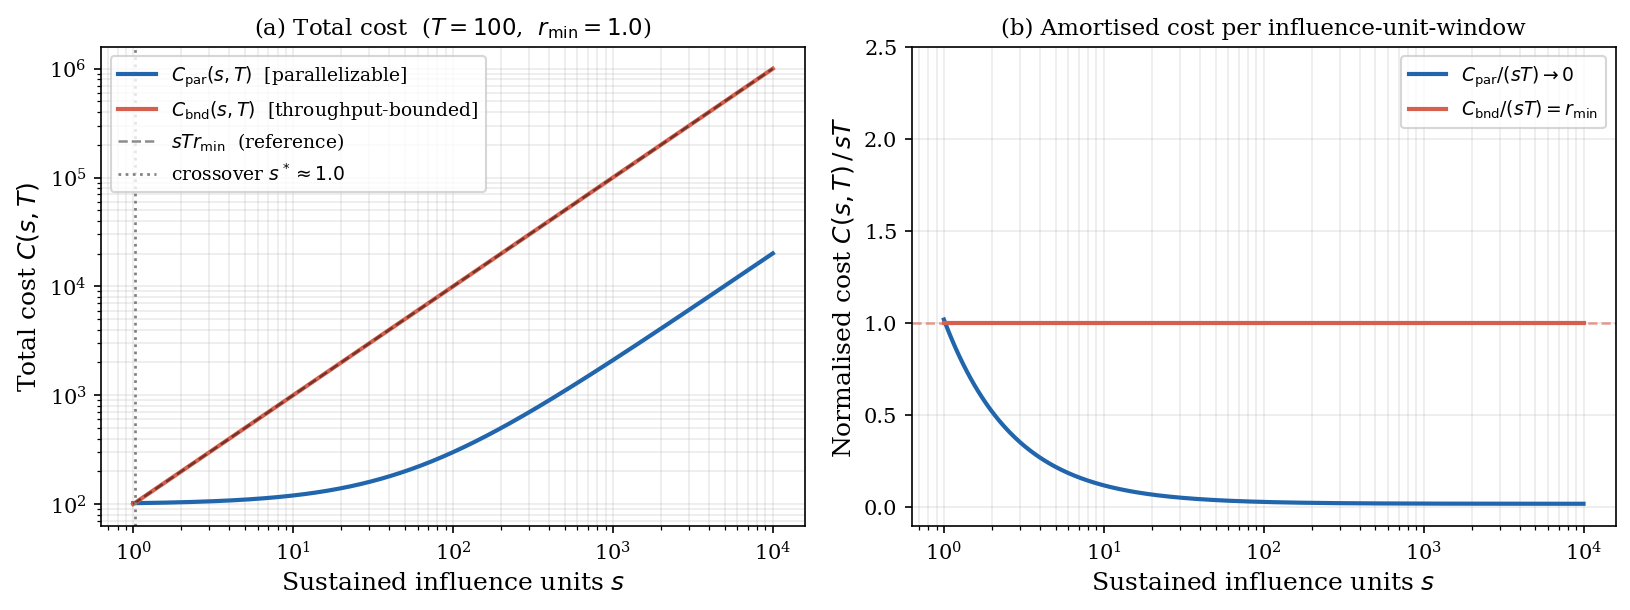
\includegraphics[width=\columnwidth]{fig1_cost_vs_s}
		\caption{Total adversarial cost $C(s,T)$ (left) and
			normalised ratio $C(s,T)/sT$ (right) vs.\ $s$,
			with $T=100$ and $r_{\min}=1.0$.
			The parallelizable ratio decays monotonically toward
			zero (Theorem~\ref{thm:impossible}); the
			throughput-bounded ratio remains fixed at $r_{\min}$
			(Theorem~\ref{thm:linear}).}
		\label{fig:cost_vs_s}
	\end{figure}
	
	Figure~\ref{fig:cost_vs_T} fixes $s=10$ and varies
	the time horizon $T$ for three values of $r_{\min}$.
	Throughput-bounded cost grows strictly linearly in $T$
	for all parameter values; parallelizable cost remains
	sublinear relative to $sT$.
	
	\begin{figure}[t]
		\centering
		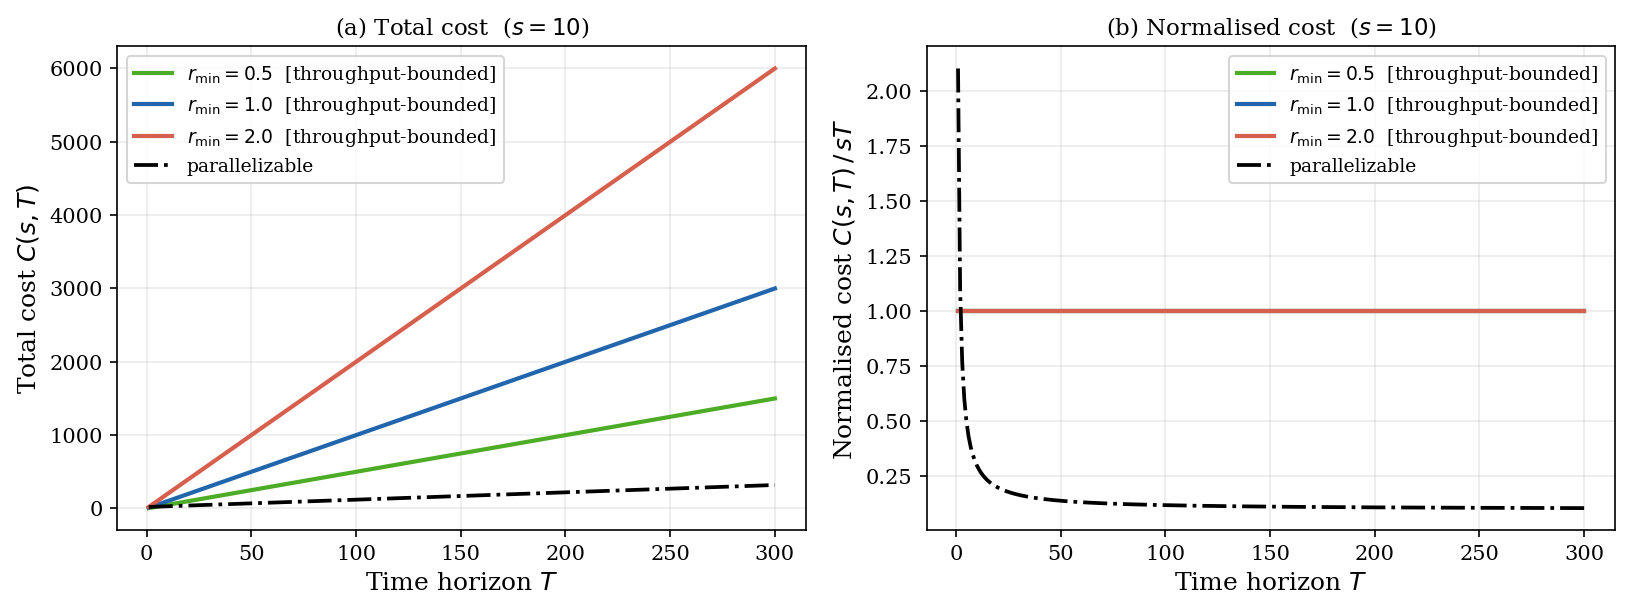
\includegraphics[width=\columnwidth]{fig2_cost_vs_T}
		\caption{Total cost (left) and normalised cost
			$C(s,T)/sT$ (right) vs.\ time horizon $T$,
			with $s=10$ and $r_{\min} \in \{0.5, 1.0, 2.0\}$.
			All throughput-bounded curves grow linearly in $T$;
			the parallelizable normalised ratio decays toward
			zero, confirming $C_{\mathrm{par}}(s,T) = o(sT)$.}
		\label{fig:cost_vs_T}
	\end{figure}
	
	%
	% --- B. ---
	%
	\subsection{Non-Amplification Under Identity Replication}
	\label{ssec:eval_nonamplification}
	
	Figure~\ref{fig:influence_share} isolates the effect
	of identity replication under a throughput-bounded
	resource.
	The honest population is fixed at $n=200$ validators.
	An adversary controls $m$ independent participation
	channels and $s$ target identities, with
	$s \in \{400, 700, 1000\}$---all strictly larger than
	the plot range of $m$.
	Adversarial influence share is
	$W_{\mathcal{A}} / W_{\mathrm{tot}} =
	\min(m,s) / (\min(m,s) + n)$.
	
	Since $s > m$ throughout, $\min(m,s) = m$ for all
	plotted values, and all three curves are identical.
	Influence share is therefore determined entirely by
	channel capacity $m$, not by identity count $s$:
	multiplying the number of adversarial identities by a
	factor of $2.5$ (from $s=400$ to $s=1000$) yields
	zero influence gain.
	This directly validates the non-amplification
	consequence of Theorem~\ref{thm:linear}.
	
	\begin{figure}[t]
		\centering
		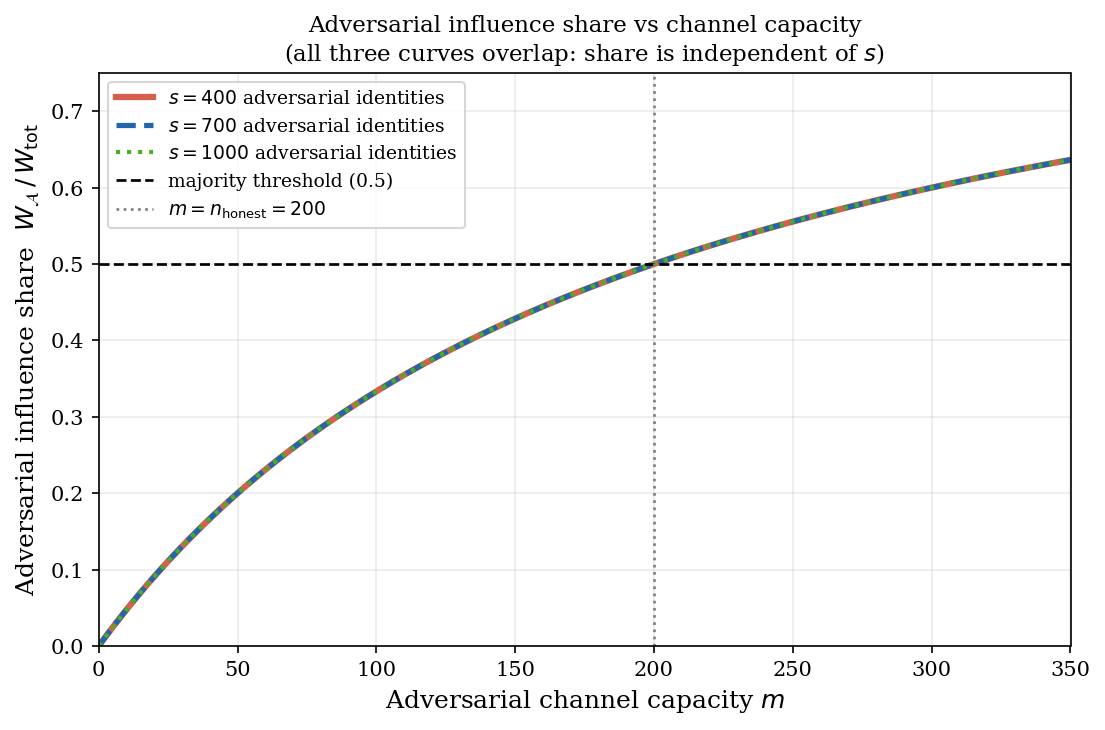
\includegraphics[width=0.92\columnwidth]{fig3_influence_share}
		\caption{Adversarial influence share vs.\ channel
			capacity $m$, for $s \in \{400, 700, 1000\}$ and
			$n_{\rm honest}=200$.
			All three curves overlap exactly: influence share
			equals $m/(m+n)$, independent of $s$.
			Identity replication without additional channel
			capacity yields no influence gain, consistent with
			Theorem~\ref{thm:linear}.}
		\label{fig:influence_share}
	\end{figure}
	
	%
	% --- C. ---
	%
	\subsection{Parameter Sensitivity}
	\label{ssec:eval_sensitivity}
	
	Table~\ref{tab:crossover} reports the crossover
	$s^*$---the value of $s$ at which
	$C_{\mathrm{bnd}}(s,T) = C_{\mathrm{par}}(s,T)$---for
	representative $(T, r_{\min})$ combinations:
	\begin{equation}
		s^* = \frac{T}{T \cdot r_{\min} - r_{\min} - 1},
		\quad T \cdot r_{\min} > r_{\min} + 1.
		\label{eq:crossover}
	\end{equation}
	For all tested values, $s^*$ is small and decreases
	as $T$ grows: by $T=25$, any adversary sustaining
	more than two or three influence units faces higher
	cost under throughput-bounded resources than under
	parallelizable ones.
	
	\begin{table}[t]
		\caption{Crossover $s^*$ for representative
			$(T, r_{\min})$ values, computed from~\eqref{eq:crossover}.
			Above $s^*$, throughput-bounded cost exceeds the
			parallelizable baseline.}
		\label{tab:crossover}
		\centering
		\renewcommand{\arraystretch}{1.2}
		\begin{tabular}{@{}rrrr@{}}
			\toprule
			$T$ & $r_{\min}=0.5$ & $r_{\min}=1.0$ & $r_{\min}=2.0$ \\
			\midrule
			10 & 2.9 & 1.2 & 0.6 \\
			25 & 2.3 & 1.1 & 0.5 \\
			50 & 2.1 & 1.0 & 0.5 \\
			100 & 2.1 & 1.0 & 0.5 \\
			200 & 2.0 & 1.0 & 0.5 \\
			\bottomrule
		\end{tabular}
	\end{table}
	
	The evaluation confirms three properties predicted
	by the theory:
	(1) the parallelizable normalised cost
	$C_{\mathrm{par}}(s,T)/sT \to 0$ as $s,T \to \infty$
	(Theorem~\ref{thm:impossible});
	(2) the throughput-bounded normalised cost
	$C_{\mathrm{bnd}}(s,T)/sT = r_{\min}$ remains bounded
	away from zero for all $s$ and $T$
	(Theorem~\ref{thm:linear});
	and (3) adversarial influence under throughput-bounded
	resources scales with channel capacity $m$, not with
	identity count $s$, confirming that identity
	replication without proportional channel capacity
	yields no influence gain.
	
	%
	% --- D. ---
	%
	\subsection{Empirical Calibration}
	\label{ssec:eval_calibration}
	
	The closed-form expressions of
	Sections~\ref{ssec:eval_cost}--\ref{ssec:eval_sensitivity}
	illustrate the asymptotic regimes using unit parameters.
	We now calibrate the model against two deployed systems
	whose concentration behavior is documented in the cited
	literature, using parameters drawn directly from those sources.
	The purpose is to show that the framework produces
	non-trivial, quantitatively grounded predictions about
	observable participation patterns.
	
	\paragraph*{Ethereum proof-of-stake}
	The Ethereum protocol requires each validator to commit
	a minimum stake of $r_{\min} = 32$~ETH~\cite{kiayias2017ouroboros},
	making this the natural activation threshold.
	As of 2023, Lido Finance operated approximately
	$s \approx 300{,}000$ validators, representing roughly
	thirty percent of all staked ETH~\cite{lido2023concentration}.
	Time is measured in epochs; one Ethereum epoch comprises
	32 slots and lasts approximately 6.4~minutes.
	
	Figure~\ref{fig:eth_calibration} applies the cost model
	to these parameters.
	Under the current parallelizable mechanism (financial
	capital), the adversarial cost is
	\[
	C_{\mathrm{par}}(300{,}000,\, T)
	\;\approx\; 9.6 \times 10^6 \;\text{ETH},
	\]
	independent of $T$: a one-time stock acquisition
	suffices regardless of the participation horizon.
	Under a hypothetical throughput-bounded mechanism with
	the same $r_{\min}$, the cost grows as
	$C_{\mathrm{bnd}}(300{,}000,\, T) = 32 \times 300{,}000 \times T$~ETH,
	reaching $9.6 \times 10^9$~ETH at $T = 1{,}000$ epochs
	(approximately 4.4~days)---a quantity exceeding the total
	circulating ETH supply by approximately two orders of
	magnitude (total supply $\approx 1.2 \times 10^8$~ETH
	as of December~2023~\cite{lido2023concentration}).
	The normalised ratio $C_{\mathrm{par}}/sT \to 0$
	while $C_{\mathrm{bnd}}/sT = r_{\min} = 32$ remains
	constant, consistent with Theorems~\ref{thm:impossible}
	and~\ref{thm:linear} respectively.
	
	\begin{figure*}[t]
		\centering
		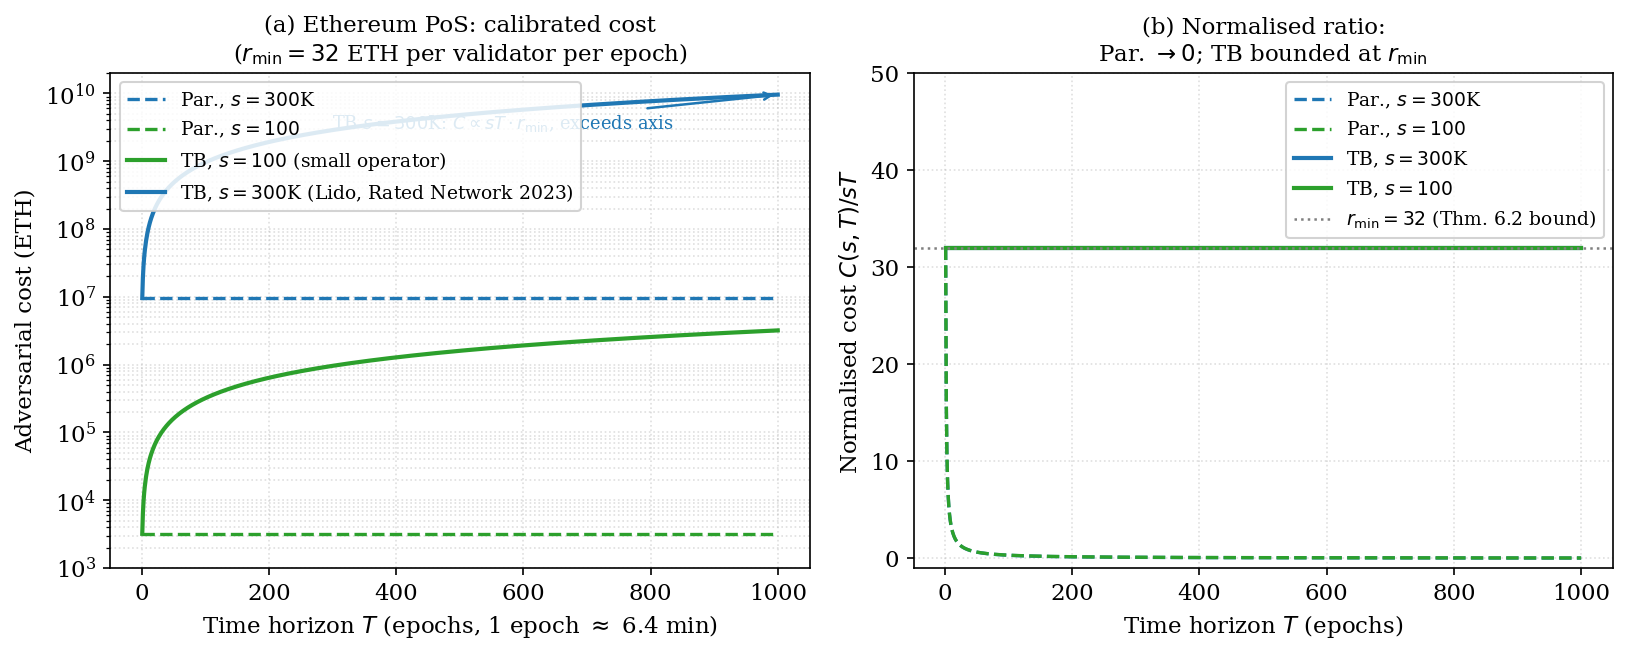
\includegraphics[width=\textwidth]{fig4_eth_calibration}
		\caption{Ethereum PoS calibration using parameters from
			Rated Network~\cite{lido2023concentration}.
			$r_{\min} = 32$~ETH; $s = 300{,}000$ (Lido tier) and
			$s = 100$ (small operator).
			\emph{Left:} total adversarial cost vs.\ time horizon
			$T$ (epochs); parallelizable cost is $T$-independent
			(Theorem~\ref{thm:impossible}), throughput-bounded cost
			scales as $\Omega(sT)$ (Theorem~\ref{thm:linear}).
			\emph{Right:} normalised ratio $C(s,T)/sT$; parallelizable
			decays to zero while throughput-bounded remains fixed at
			$r_{\min}$.}
		\label{fig:eth_calibration}
	\end{figure*}
	
	\paragraph*{Bitcoin proof-of-work}
	Gencer et al.~\cite{gencer2018decentralization} report that
	the top-four Bitcoin mining pools collectively controlled
	over fifty percent of total hash power, with individual
	shares of approximately $16.5\%$, $15.5\%$, $12.0\%$,
	and $11.5\%$, respectively.
	We represent each pool's effective identity count
	proportional to its share of a normalised network of
	$N = 10{,}000$ units.
	
	Figure~\ref{fig:btc_calibration}(a) plots
	$C_{\mathrm{par}}(s,T)/sT$ for four operator tiers
	spanning small pools ($s = 50$) to the top-pool tier
	($s = 1{,}650$).
	For all tiers, the ratio decays toward zero as $T$ grows,
	confirming the $C_{\mathrm{par}}(s,T) = o(sT)$ prediction
	of Theorem~\ref{thm:impossible}.
	Figure~\ref{fig:btc_calibration}(b) displays the marginal
	cost separation: $\Delta_{\mathrm{par}}(s,T) = O(1)$
	versus $\Delta_{\mathrm{bnd}}(s,T) = \Omega(T)$,
	illustrating the structural gap of
	Theorem~\ref{thm:separation}.
	
	\begin{figure*}[t]
		\centering
		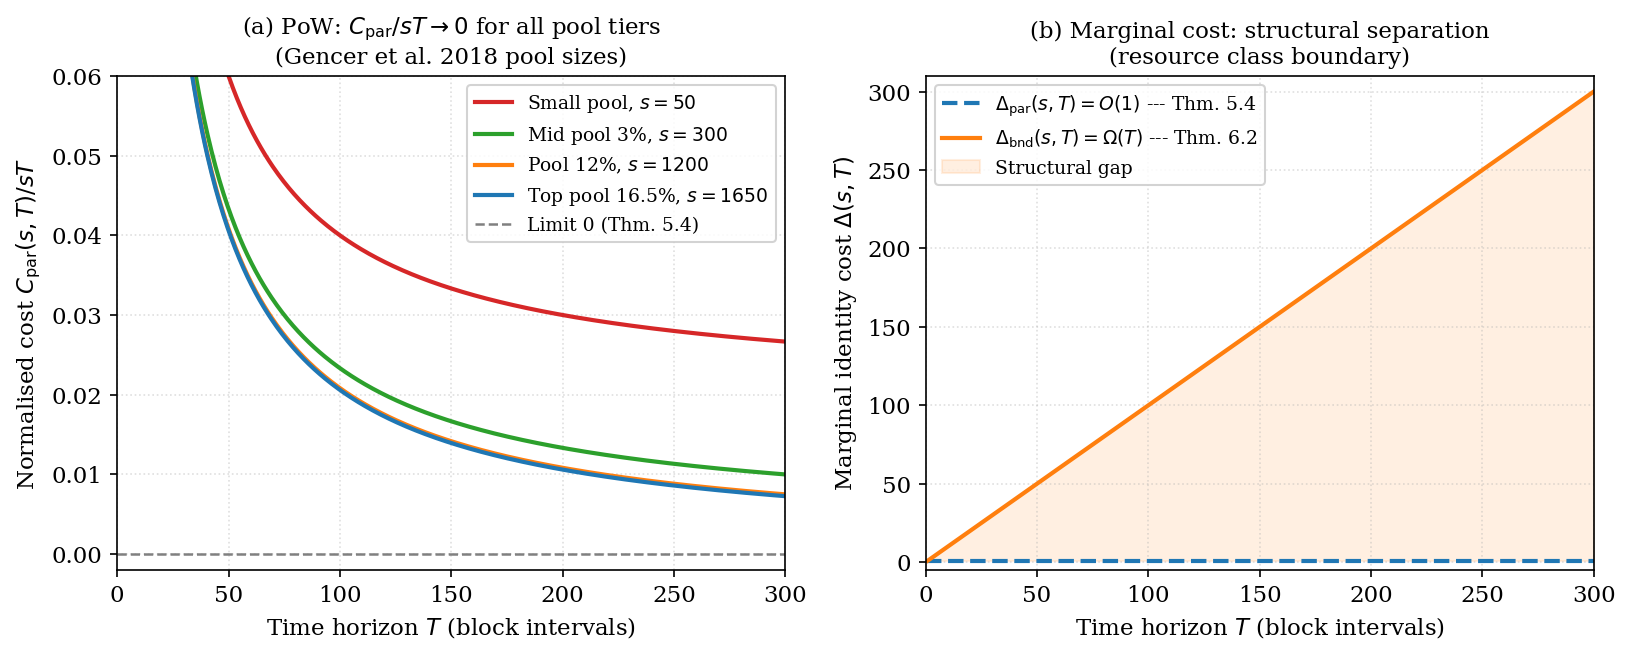
\includegraphics[width=\textwidth]{fig5_btc_calibration}
		\caption{Bitcoin PoW calibration using pool share data
			from Gencer et al.~\cite{gencer2018decentralization}.
			\emph{Left:} normalised cost $C_{\mathrm{par}}(s,T)/sT$
			for four operator tiers; all decay toward zero
			(Theorem~\ref{thm:impossible}), with larger pools
			converging faster.
			\emph{Right:} marginal cost $\Delta(s,T)$ under each
			resource class; the structural gap between $O(1)$ and
			$\Omega(T)$ regimes across the full time horizon
			(Theorem~\ref{thm:separation}).}
		\label{fig:btc_calibration}
	\end{figure*}
	
	The calibration confirms that the asymptotic separation
	of Theorems~\ref{thm:impossible} and~\ref{thm:linear}
	is not merely a theoretical asymptote: at the scale of
	deployed systems and realistic participation horizons,
	the cost gap between parallelizable and throughput-bounded
	mechanisms is quantitatively decisive.
	For the Lido-scale case, the crossover occurs within the
	first few epochs; for Bitcoin pool tiers, within the first
	few hundred block intervals.
	
	
	
	% -------------------------------------------------------
	%  X. LIMITATIONS AND OPEN PROBLEMS
	% -------------------------------------------------------
	\section{Limitations and Open Problems}
	\label{sec:limitations}
	
	The structural separation established in this paper
	characterizes adversarial cost scaling under explicit
	modeling assumptions.
	Several limitations and open directions remain.
	
	%
	% --- A. ---
	%
	\subsection{Enforcement of Throughput Constraints}
	\label{ssec:lim_enforcement}
	
	The framework assumes a per-identity throughput bound
	$\tau$ and activation threshold $r_{\min}$ that hold
	structurally.
	Practical mechanisms approximate non-transferability
	and window-locality via device attestation and session
	serialization, but no deployment enforces them perfectly;
	advances in automation may effectively increase $\tau$.
	The formal guarantees hold given the structural
	properties of Definitions~\ref{def:parallelizable}
	and~\ref{def:throughput}; deployment-level fidelity
	is outside the scope of the present framework.
	
	%
	% --- B. ---
	%
	\subsection{Non-Additive Hybrid Compositions}
	\label{ssec:lim_hybrid}
	
	Lemma~\ref{lem:hybrid} establishes that a
	throughput-bounded component preserves the linear
	lower bound under \emph{additive} cost decomposition.
	Non-additive compositions---where the two resource
	classes interact in ways that are not captured by
	$C(s,T) = C_p(s,T) + C_t(s,T)$---remain outside
	the present scope.
	
	For example, a system might require a minimum threshold
	of both parallelizable and throughput-bounded resources
	to be active, creating a non-additive coupling.
	Whether the linear lower bound is preserved under
	such compositions is an open problem.
	
	%
	% --- C. ---
	%
	\subsection{Economic Coordination and Identity Markets}
	\label{ssec:lim_markets}
	
	The model abstracts away economic coordination dynamics.
	In practice, delegation markets, identity outsourcing,
	and secondary markets for rate-limited credentials may
	alter the effective cost structure; characterizing
	equilibrium behavior under adaptive incentives and
	strategic outsourcing remains outside the present scope.
	
	%
	% --- D. ---
	%
	\subsection{Window Granularity and Temporal Modeling}
	\label{ssec:lim_windows}
	
	The model partitions time into discrete windows of
	fixed duration.
	Smaller windows increase renewal frequency under
	throughput-bounded resources; larger windows may weaken
	window-local constraints.
	A window-independent formulation expressing the
	separation in terms of wall-clock time remains an
	open direction.
	
	%
	% --- E. ---
	%
	\subsection{Scope of the Framework}
	\label{ssec:lim_scope}
	
	The framework is structural and protocol-agnostic:
	it characterizes the resource-level preconditions
	that any mechanism must satisfy, and does not replace
	deployment-specific security analyses, probabilistic
	consensus proofs, or economic equilibrium models.
	Characterizing intermediate scaling regimes---where
	structural properties are only partially satisfied---in
	full generality remains an open theoretical problem.
	
	
	% -------------------------------------------------------
	%  XI. CONCLUSION
	% -------------------------------------------------------
	\section{Conclusion}
	\label{sec:conclusion}
	
	Binding influence to a scarce resource prevents cheap
	identity creation from amplifying adversarial power---
	but scarcity alone is insufficient.
	The structural properties of the resource determine
	whether influence can be concentrated at sublinear
	cost, regardless of how the protocol is designed.
	
	We proved that any resource satisfying divisibility,
	additivity of influence, temporal reusability, and
	identity transferability admits influence amortization:
	$C(s,T) = o(sT)$, with marginal cost $\Delta(s,T) = O(1)$
	that does not grow with the time horizon
	(Theorem~\ref{thm:impossible}).
	This is an impossibility result: no protocol rule can
	enforce linear cost of influence concentration over
	a structurally parallelizable resource.
	We further proved that throughput-bounded,
	non-transferable, window-local resources enforce
	$C(s,T) = \Omega(sT)$, with marginal cost
	$\Delta(s,T) = \Omega(T)$ growing with the time horizon
	(Theorem~\ref{thm:linear}).
	Theorems~\ref{thm:impossible} and~\ref{thm:linear}
	together establish a sharp asymptotic separation
	between the two resource classes
	(Theorem~\ref{thm:separation}).
	
	The Resource Substitution Principle
	(Theorem~\ref{thm:substitution}) translates this
	separation into a design rule: enforcing linear
	cost of influence concentration requires grounding
	participation in a resource that violates at least
	one parallelizability property.
	Protocol design cannot substitute for resource
	structure.
	Any mechanism grounded in a throughput-bounded,
	non-transferable, and window-local resource inherits
	$C(s,T) = \Omega(sT)$ by construction---without
	additional protocol-level enforcement.
	
	Future directions include the formal characterization
	of intermediate scaling regimes under partial
	violations of parallelizability, equilibrium analysis
	under adaptive incentives and identity markets, and
	the design of practical mechanisms that enforce
	throughput-boundedness while preserving
	permissionlessness and accessibility.
	
	
	% -------------------------------------------------------
	%  APPENDICES
	% -------------------------------------------------------
	%\appendices
	
	%\section{Tightness of the Scaling Bounds}
	%\label{app:tightness}
	% Both regimes are asymptotically tight.
	% Parallelizable: C(s,T) <= s*rmin + h(s,T) -> 0/sT
	% Throughput-bounded: rv(t) = rmin => C(s,T) = Theta(sT)
	
	%\section{Robustness Under Extended Adversarial Models}
	%\label{app:robustness}
	% Adaptive identity creation
	% Coalitions
	% Stochastic throughput: E[C(s,T)] = Omega(sT)
	
	\bibliographystyle{IEEEtran}
	\bibliography{references}
	
	
	
	
\end{document}